\frame
{
\frametitle{Introduction}
\begin{enumerate}
\item Nonparametric bootstrap estimates
\item Example of failure of the nonparametric bootstrap estimate 
\item Parametric Bootstrap
\item Resampling and Monte Carlo Sampling
\item The law school example
\end{enumerate}
}
%%%%%%%%%%%%%%%%%%%%%%%%%%%%%%%%%%%%%%%%%%%%%%%%%%%%%%%%
%%%%%%%%%%%%%%%%%%%%%%%%%%%%%%%%%%%%%%%%%%%%%%%%
\frame{
\frametitle{Non-Parametric Bootstrap}

\begin{figure}[!h]
$$
\begin{array}{rcr}
Real\ World & & Bootstrap\ World \\
&&\\
f \rightarrow \mathbf{x}  & \Rightarrow & \hat{f} \rightarrow \mathbf{x}^{*} \\
&&\\
\downarrow & & \downarrow \ \\
&&\\
\hat{\theta} & & \hat{\theta}^{*}\\
\end{array} 
$$
\caption{Unknown probability model $f$ gives observed data $\mathbf{x}$ and we wish to know the accuracy of the statistic $\hat{\theta}=s(\mathbf{x})$ for estimating the parameter of interest $\theta=t(f)$. No prior information is available on $f$, therefore $\hat{f}$ is estimated from $\mathbf{x}$ as the empirical distribution function. Accuracy is inferred from observed variability of bootstrap replication $\hat{\theta}^{*}=s(\mathbf{x}^{*})$.}
\end{figure}

}

%%%%%%%%%%%%%%%%%%%%%%%%%%%%%%%%%%%%%%%%%%%%%%%%%%%%%%%%
%%%%%%%%%%%%%%%%%%%%%%%%%%%%%%%%%%%%%%%%%%%%%%%%%%%%%%%%%%%%%%
\frame{
\frametitle{Convergence of the bootstrap estimates}

\begin{exampleblock}{Example A}
  $f(x)=0.2\ \mathcal{N}(\scriptstyle \mu=1,\sigma=2 \displaystyle) +0.8\  \mathcal{N}( \scriptstyle\mu=6,\sigma=1 \displaystyle)$ $\leadsto$ $\mathbf{x}=(x_1,\cdots,x_{100})$.
\end{exampleblock}
\begin{figure}[!h]
\begin{tabular}{cc}
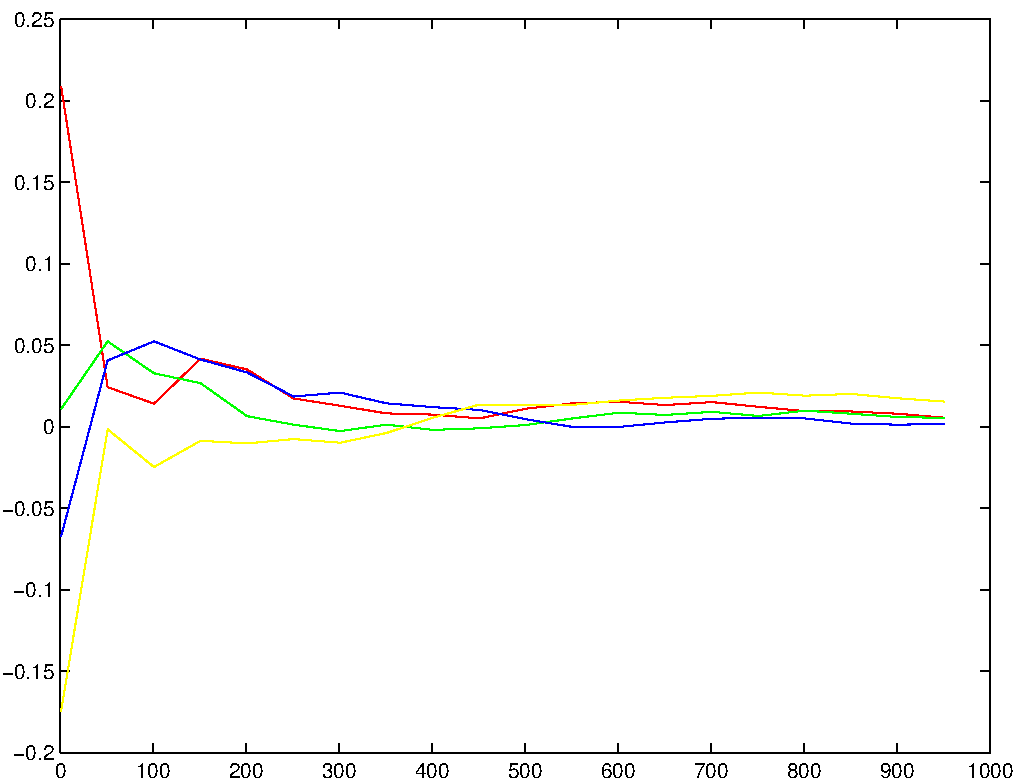
\includegraphics[width=.4\linewidth]{biasExA} &
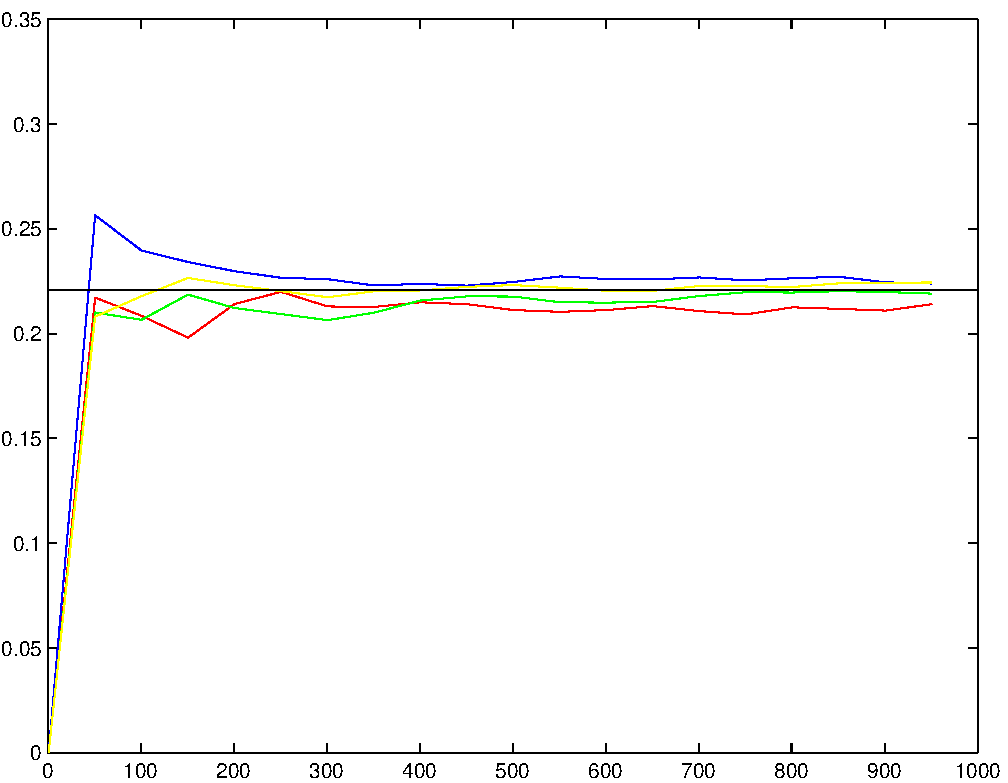
\includegraphics[width=.4\linewidth]{stdExA} \\ 
$\widehat{\mathrm{Bias}}$ & $\hat{se}_{B}$ \\
\end{tabular}
\caption{Bias and standard error bootstrap estimates w.r.t. $B$ (4 experiments have been run).}
\end{figure}

%\begin{block}{}
%you usually need to compute more $B$ bootstrap resamples to compute the bootstrap bias estimate than the bootstrap standard error. 
%\end{block}
}

%%%%%%%%%%%%%%%%%%%%%%%%%%%%%%%%%%%%%%%%%%%%%%%%%%%%%%%%%%%%%%
\frame{
\frametitle{Example of non-parametric bootstrap failure}

\begin{exampleblock}{Example B}
Considering a sample $\mathbf{x}$ drawn from a uniform  distribution $f=\mathcal{U}(0,\theta=1)$, the statistics of interest is $\hat{\theta}=\max\lbrace x_1,\cdots,x_n\rbrace$, and ${\scriptstyle\mathbf{x}=(0.5729, 0.1873, 0.5984,  0.2883,    0.8722,}$
${\scriptstyle 0.4320,    0.4896,    0.7106, 0.2754 ,   0.7637)}$.
%Assuming that $\hat{\theta}=x_1$ and that all $x_i$s are different, the probability of a replication $\hat{\theta}^{*}$ to be equal to $x_1$ is 0.632. 
\end{exampleblock}

\begin{columns}[t]
\column{.45\linewidth}
\begin{figure}[!h]
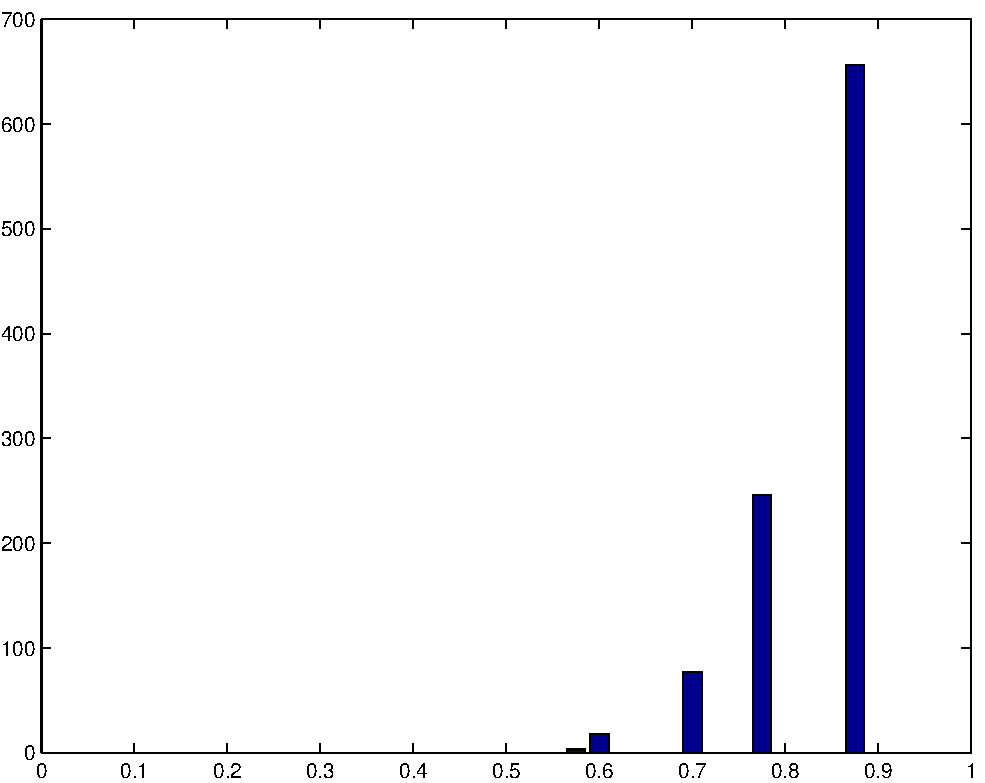
\includegraphics[width=.7\linewidth]{UniformNP.pdf} 
\caption{\tiny{Histogram of the nonparametric bootstrap replications $\hat{\theta}^{*}$ with $n=10$, $B=1000$, $\hat{\theta}=0.8722$. The maximum peak is at $\hat{\theta}=0.8722$ with a probability of $\mathcal{P}(\hat{\theta}\in \mathbf{x}^{*})= 0.6560 \approx 1-\left(1-1/n\right)^{n}= 0.6513$.}}
\end{figure} 
\column{.5\linewidth}
\begin{figure}[!h]
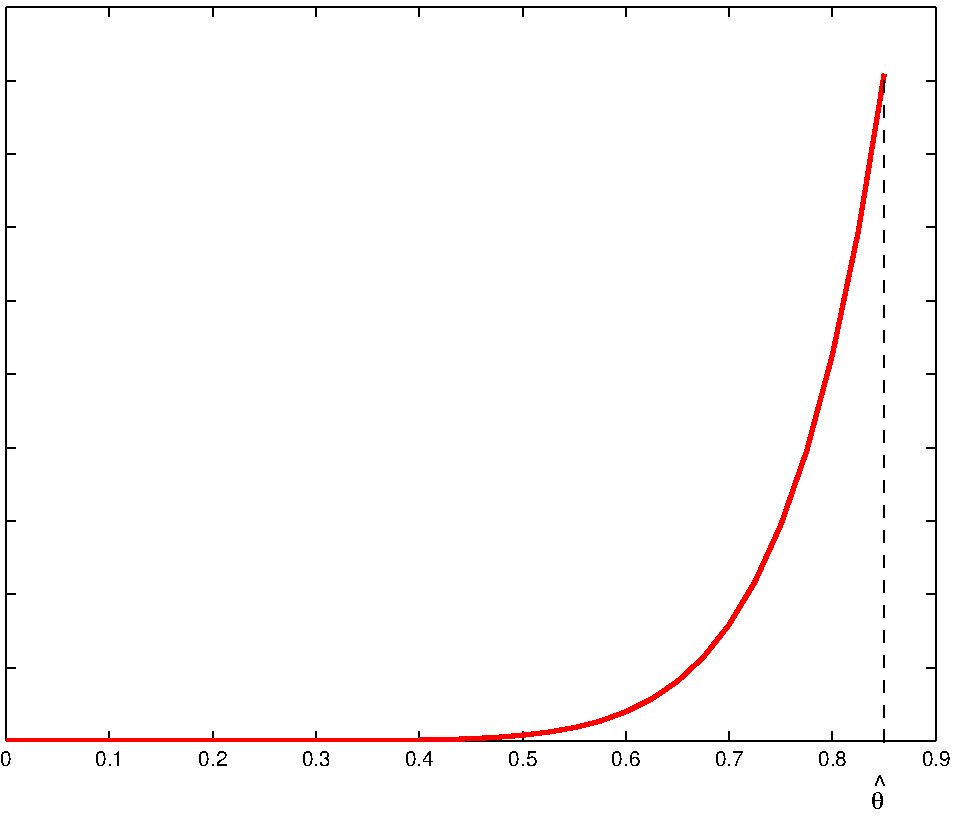
\includegraphics[width=.6\linewidth]{idealUniform.pdf} 
\caption{\tiny{Theoretical results (extreme values) says that $\mathcal{P}(\hat{\theta}^{*})=n \frac{(\hat{\theta}^{*})^{n-1}}{\hat{\theta}^{n}}$.}}
\end{figure} 
\end{columns}
}
%%%%%%%%%%%%%%%%%%%%%%%%%%%%%%%%%%%%%%%%%%%%%%%%%%%%%%%%%%%%%%
\frame{
\frametitle{Example of non-parametric bootstrap failure}
\begin{exampleblock}{Example B}
What went wrong in this example ?
\begin{itemize}
\item The empirical density function  $\hat{f}$ is not a good approximation of the true distribution $f=\mathcal{U} (0,\theta)$.

\

\item Either parametric knowledge of $f$ or some smoothing of $\hat{f}$ is needed to rectify matters.

\end{itemize}
\end{exampleblock}
}
%%%%%%%%%%%%%%%%%%%%%%%%%%%%%%%%%%%%%%%%%%%%%%%%%%%%%%%%
\frame{
\frametitle{Convergence of the bootstrap estimates}
With $\mathbf{x}=(x_1,\cdots,x_n)$, $n$ i.i.d. values, it is required:\

\

\begin{enumerate}
\item Convergence of $\hat{f}$ to $f$ for $n \rightarrow \infty$ (Glivenko-Cantelli lemma)\

\

\item Estimate $\hat{\theta}=t(\hat{f})$ is the plug-in estimate of $\theta=t(f)$\

\

\item Smoothness condition on the functional. E.g
\begin{itemize}
\item  Smooth functionals: means, variance, etc.
\item Not smooth: extreme order statistics (minimum, maximum)
\end{itemize}
\end{enumerate}
}
%%%%%%%%%%%%%%%%%%%%%%%%%%%%%%%%%%%%%%%%%%%%%%%%%%%%%%%%%%%%%%
%%%%%%%%%%%%%%%%%%%%%%%%%%%%%%%%%%%%%%%%%%%%%%%%%%%%%%%%
\frame
{
\frametitle{Parametric Bootstrap}

\begin{figure}[!h]
$$
\begin{array}{rcccr}
Real\ World & & Estimation & & Bootstrap\ World \\
&&&&\\
Prior: f\simeq \mathcal{N}(\mu,\sigma) \rightarrow \mathbf{x}  & \Rightarrow & (\overline{x},\hat{\sigma})& & \hat{f}\simeq\mathcal{N}(\overline{x},\hat{\sigma}) \rightarrow \mathbf{x}^{*} \\
&&&&\\
\downarrow &&& & \downarrow \ \\
&&&&\\
\hat{\theta} && & & \hat{\theta}^{*}\\
\end{array} 
$$
\caption{Example of parametric Bootstrap. $f$ is a normal distribution of unknown parameters $(\mu, \sigma)$. From the observed data $\mathbf{x}$ drawn from $f$, an estimation of the parameters  is performed giving $(\overline{x},\hat{\sigma})$.
$\hat{f}$ is then modelled by a normal distribution $\mathcal{N}(\overline{x},\hat{\sigma})$, from which bootstrap replications can be drawn $\mathbf{x}^{*}$.  Accuracy is inferred from observed variability of bootstrap replication $\hat{\theta}^{*}=s(\mathbf{x}^{*})$.}
\end{figure}
}

%%%%%%%%%%%%%%%%%%%%%%%%%%%%%%%%%%%%%%%%%%%%%%%%%%%%%%%%%%%%%%
\frame
{
\frametitle{Example with extreme value}
\begin{columns}[c]
\column{.45\linewidth}
\begin{exampleblock}{Example B}
We draw $B=1000$ bootstrap replication of $\hat{\theta}^{*}=\max \lbrace \mathbf{x}^{*}\rbrace$ using the parametric assumption $\mathcal{U}(0,\hat{\theta})$.

The extreme value distribution is  $\mathcal{P}(\hat{\theta}^{*})=n \frac{(\hat{\theta}^{*})^{n-1}}{\hat{\theta}^{n}}$. 
\end{exampleblock}

\column{.45\linewidth}

\begin{figure}[!h]
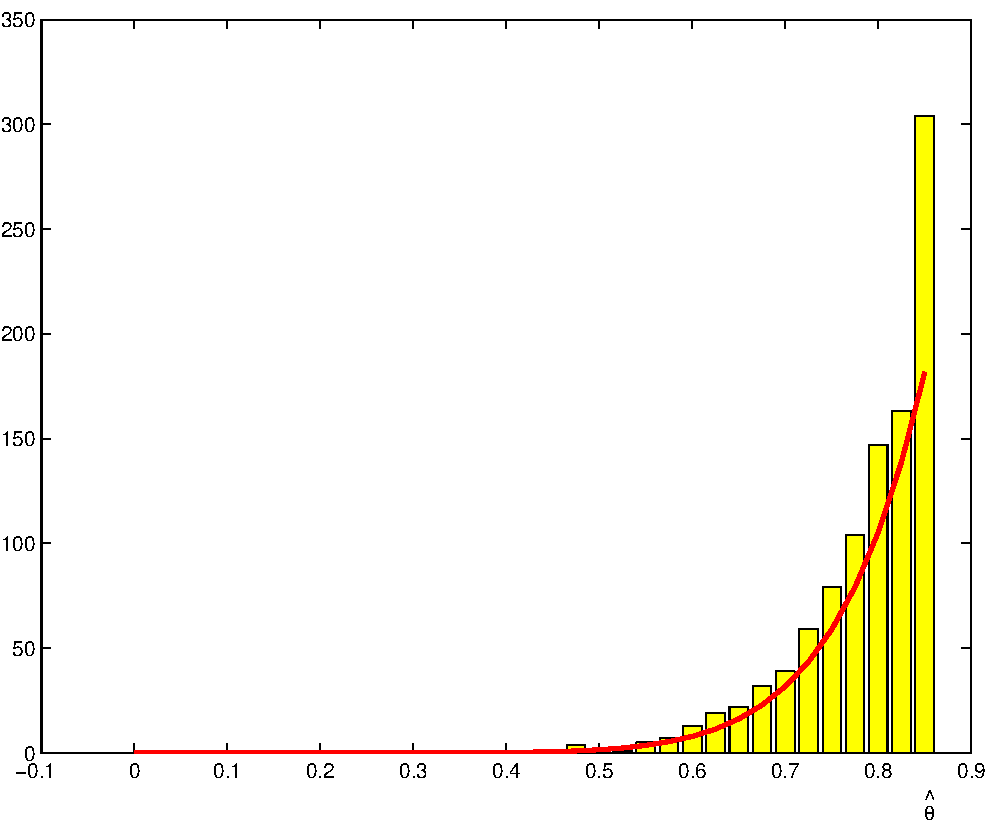
\includegraphics[width=.9\linewidth]{UniformP.pdf} 
\caption{Histogram of the parametric bootstrap replications $\hat{\theta}^{*}$ with $n=10$, $B=1000$, $\hat{\theta}=0.8722$.}
\end{figure} 

\end{columns}
}
%%%%%%%%%%%%%%%%%%%%%%%%%%%%%%%%%%%%%%%%%%%%%%%%%%%%%%%%%%%%%%
%%%%%%%%%%%%%%%%%%%%%%%%%%%%%%%%%%%%%%%%%%%%%%%%%%%%%%%%%%%%%%
\frame
{
\frametitle{The Law school example}

%\small
\begin{table}[!h]
\begin{flushleft}
\begin{tabular}{lcccccccc}
School &   1  &   2 &    3   &  4  &   5  &   6   &  7  &   8  \\
\hline
LSAT (X) & 576  &  635  &  558 &   578  &  666  &  580  &  555   & 661  \\
GPA (Y) &  3.39   &  3.30   &  2.81   &  3.03  &   3.44   &  3.07   &  3.00   &  3.43 \\

&&&&&&&&\\
\end{tabular}

\begin{tabular}{lccccccc}

School &       9   & 10   & 11 &   12  &  13  &  14   & 15 \\
\hline
LSAT (X) &  651   & 605  &  653  &  575   & 545  &  572  &  594 \\
GPA (Y) &    3.36   &  3.13  &   3.12  & 2.74   &  2.76   &  2.88   &  2.96\\

\end{tabular}
\end{flushleft}
\caption{Results of law schools admission practice  for the LSAT and GPA tests. It is believed that these scores are highly correlated. \alert{Compute the correlation and its standard error.}}
\end{table}


}



\frame
{
\frametitle{Correlation}
The correlation is defined :
$$ 
\mathrm{corr}(X,Y)=\frac{\mathbb{E}\lbrack (X -\mathbb{E}(X)) \cdot (Y -\mathbb{E}(Y))\rbrack }{\left( \mathbb{E} \lbrack (X -\mathbb{E}(X))^2 \rbrack  \cdot \mathbb{E} \lbrack (Y -\mathbb{E}(Y))^2 \rbrack \right)^{1/2}}
$$ 

Its typical estimator is:
$$
\widehat{\mathrm{corr}}(\mathbf{x},\mathbf{y})=\frac{\sum_{i=1}^{n} x_i\ y_i - n\ \overline{x}\ \overline{y}}{\lbrack \sum_{i=1}^{n}x_i^2-n\overline{x}^2 \rbrack^{1/2}\cdot \lbrack\sum_{i=1}^{n} y_i^2-n \overline{y}^2 \rbrack^{1/2} }
$$

}

%
\frame{
\frametitle{The Law school example}
\begin{itemize}
\item The estimated correlation is $\widehat{\mathrm{corr}}(\mathbf{x},\mathbf{y})=.7764$ between LSAT and GPA. 
%\item Precise theoretical formula for the standard error of the estimator is unavailable.
\end{itemize}
\begin{exampleblock}{Non-parametric Bootstrap estimate of the standard error}

\begin{table}[!h]
\begin{tabular}{l|cccccccc}
$B$ & 25 & 50 & 100 & 200 & 400 & 800 & 1600 & 3200 \\
\hline
$\hat{\mathrm{se}}_B$& .140 & .142 & .151 & .143 & .141 &.137 & .133 & .132 \\
\end{tabular}
\caption{Bootstrap estimate of standard error for $\widehat{\mathrm{corr}}(\mathbf{x},\mathbf{y})=.776$.}
\end{table}
The standard error stabilizes to $\mathrm{se}_{\hat{f}} (\widehat{\mathrm{corr}})\approx.132$.  
\end{exampleblock}
}

%%%%%%%%%%%%%%%%%%%%%%%%%%%%%%%%%%%%%%%%%%%%%%%%%%%
\frame
{
\frametitle{The Law school example}

\begin{columns}[t]
\column{0.5\linewidth}
\begin{exampleblock}{Parametric Bootstrap approach}
Assuming  that $f$ is a bivariate normale distribution, $\hat{f}_{norm}$ is estimated by computing the mean $\overline{\mathbf{z}}=(\overline{x},\overline{y})$ and the covariance matrix $\widehat{\Sigma}$ from the data.

Then $B$ samples $(\mathbf{x},\mathbf{y})^{*}$ %(of size $n=15$)
 can be drawn from $\hat{f}_{par}$ and the bootstrap estimate of the correlation coefficient can be performed. 

%$\overline{x}=600.2667$ and $\overline{y}= 3.0947$ and 
%$$ 
%\hat{\Sigma}=
%\left \lbrack
%\begin{array}{cc}
%2445  & 110.6 \\
%110.6 & 0.8302\\
%\end{array}
%\right\rbrack
%$$

\end{exampleblock}
\column{0.5\linewidth}
\begin{figure}[!h]
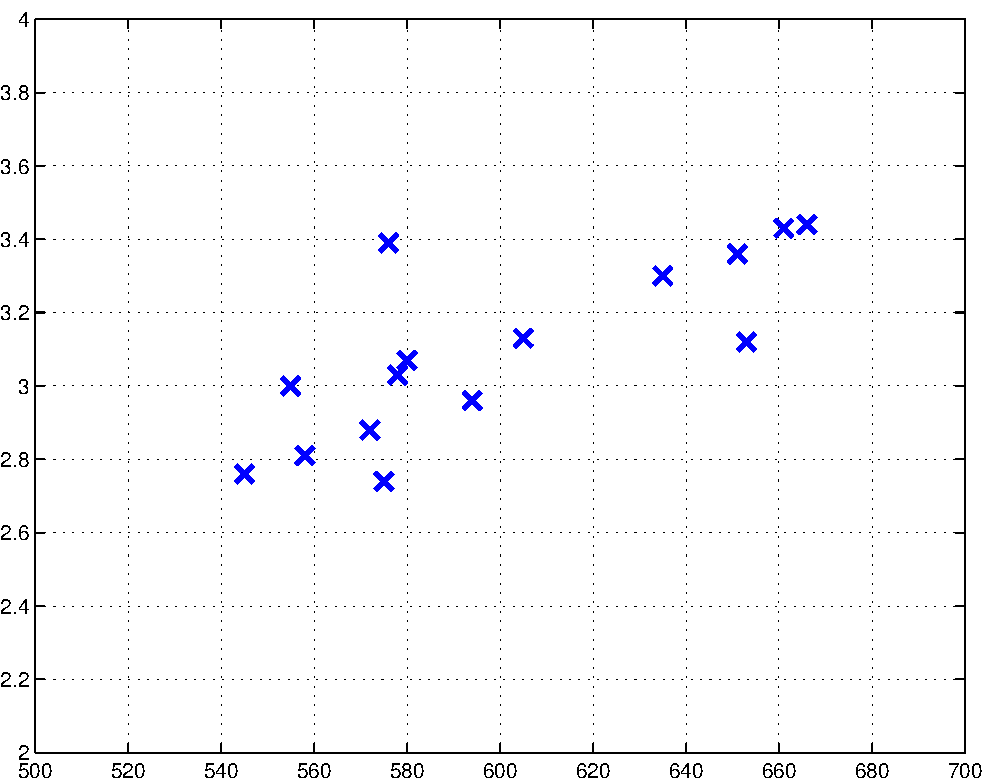
\includegraphics[width=.9\linewidth]{schoollsatgpa}
\end{figure}
\end{columns}

}


%%%%%%%%%%%%%%%%%%%%%%%%%%%%%%%%%%%%%%%%%%%%%%%%%%%%%%%%
\frame
{
\frametitle{The Law school example: Parametric Approach}

\begin{exampleblock}{Prior model}
\begin{itemize}
\item \textbf{Assumption.} $f$ is a bivariate normal density function of the form:
$$ 
f(x,y)=\frac{\exp\left\lbrack -\frac{(\mathbf{z}-\pmb{\mu}_{zf})^{T} \Sigma^{-1} (\mathbf{z}-\pmb{\mu}_{zf})}{2} 
\right\rbrack
}{(2\pi) |\det(\Sigma)|^{1/2}}
$$ 
with 
$
\mathbf{z}=
\left(
\begin{array}{c}
x\\
y\\
\end{array}\right)
$
\item \textbf{Problem.} The parameters, mean  $\pmb{\mu}_{zf}=(\mu_{xf},\mu_{yf})$ and  the covariance matrix $\Sigma$, are unknown. 
\end{itemize}
\end{exampleblock}
}

%%%%%%%%%%%%%%%%%%%%%%%%%%%%%%%%%%%%%%%%%%%%%%%%%%%%%%%%%
\frame
{
\frametitle{The Law school example: Parametric Approach}

\begin{exampleblock}{Estimate of the parametric p.d.f.}


The parametric  p.d.f. is estimated by:
$$ 
\hat{f}_{par}(x,y)=\frac{\exp\left\lbrack -\frac{(\mathbf{z}-\overline{\mathbf{z}})^{T} \overline{\Sigma}^{-1} (\mathbf{z}-\overline{\mathbf{z}})}{2} 
\right\rbrack
}{(2\pi) |\det(\overline{\Sigma})|^{1/2}}
$$
Means are $\overline{\mathbf{z}}=(\overline{x}=\frac{\sum_{i=1}^n x_i}{n},\overline{y}=\frac{\sum_{i=1}^n y_i}{n})$. 
The covariance matrix is defined as:
$$
\overline{\Sigma}=\frac{1}{n-1} \left\lbrack
\begin{array}{cc}
\sum_{i=1}^{n} (x_i-\overline{x})^2 & \sum_{i=1}^{n} (x_i-\overline{x})  (y_i-\overline{y})\\
&\\
\sum_{i=1}^{n} (x_i-\overline{x})  (y_i-\overline{y}) & \sum_{i=1}^{n} (y_i-\overline{y})^2 \\
\end{array}
\right\rbrack
$$
The mean is $\overline{\mathbf{z}}=(\overline{x}=600.3,\overline{y}=3.1)$ and
$
\overline{\Sigma}=
\left\lbrack
\begin{array}{cc}
1747 & 0.0079\\
0.0079 & 0.0001\\
\end{array}
\right\rbrack
$
\end{exampleblock}
}
%%%%%%%%%%%%%%%%%%%%%%%%%%%%%%%%%%%%%%%%%%%%%%%%%%%%%%%%
\frame{
\frametitle{Parametric Bootstrap estimate of standard error}

\begin{beamercolorbox}[wd=\linewidth, rounded=true,shadow=true]{postit}
\begin{enumerate}
\item Using the prior assumption and the available observation $\mathbf{x}=(x_1,x_2,\cdots,x_n)$, estimate $\hat{f}_{par}$
\item Instead of sampling with replacement from the data $\mathbf{x}$, draw $B$ samples $\mathbf{x}^{*(b)}$ of size $n$ from $\hat{f}_{par}$
\item Evaluate the bootstrap replications:
$$ 
\hat{\theta}^{*}(b)=s(\mathbf{x}^{*(b)}), \quad \forall b \in \lbrace 1,\cdots,B \rbrace
$$

\item Estimate the standard error $\mathrm{se}_{f}(\hat{\theta})$ by the standard deviation of the $B$ replications:
$$ 
\hat{\mathrm{se}}_{B}=\left\lbrack \frac{\sum_{b=1}^{B}\lbrack \hat{\theta}^{*}(b)-\hat{\theta}^{*}(\cdot)\rbrack^{2}}{B-1} \right\rbrack^{\frac{1}{2}}
$$
where $\hat{\theta}^{*}(\cdot)=\frac{\sum_{b=1}^{B} \hat{\theta}^{*}(b)}{B}$.
\end{enumerate}
\end{beamercolorbox}
}

%%%%%%%%%%%%%%%%%%%%%%%%%%%%%%%%%%%%%%%%%%%%%%%%%%%%%%%%
\frame{
\frametitle{Parametric Bootstrap estimate of the bias}

\begin{beamercolorbox}[wd=\linewidth, rounded=true,shadow=true]{postit}
\begin{enumerate}
\item Using the prior assumption and the available observation $\mathbf{x}=(x_1,x_2,\cdots,x_n)$, estimate $\hat{f}_{par}$
\item Instead of sampling with replacement from the data $\mathbf{x}$, draw $B$ samples $\mathbf{x}^{*(b)}$ of size $n$ from $\hat{f}_{par}$
\item Evaluate the bootstrap replications:
$$ 
\hat{\theta}^{*}(b)=s(\mathbf{x}^{*(b)}), \quad \forall b \in \lbrace 1,\cdots,B \rbrace
$$

\item Estimate the bias: 
$$ 
\widehat{\mathrm{Bias}}_{B}=\hat{\theta}^{*}(\cdot)-\hat{\theta}
$$
where $\hat{\theta}^{*}(\cdot)=\frac{\sum_{b=1}^{B} \hat{\theta}^{*}(b)}{B}$.
\end{enumerate}
\end{beamercolorbox}
}
%%%%%%%%%%%%%%%%%%%%%%%%%%%%%%%%%%%%%%%%%%%%%%%%%%%%%%%%
\frame{
\frametitle{Resampling and Monte Carlo Simulation}

\begin{itemize}
\item  In resampling, one could do all possible combinations, but it would be too time-consuming and computing-intensive. \

\

\item The alternative is Monte Carlo sampling, which restricts the resampling to a certain number. It is used in the computation of the bootstrap samples in the nonparametric case when a random index $(i_1,\cdots,i_n)$ is simulated from the uniform distribution $[1;n]$ ($\mathbf{x}^{*}=(x_{i_1},\cdots,x_{i_1})$). 

\

\item The data could be totally hypothetical in Monte Carlo simulation, while in the resampling,  the simulation is based upon some real observation $\mathbf{x}=(x_1,\cdots,x_n)$.

\

\item In the parametric case, the bootstrap samples from $\hat{f}_{par}$ are computed using Monte Carlo methods and are not anymore resamples from $\mathbf{x}$.  

\end{itemize}
}
%%%%%%%%%%%%%%%%%%%%%%%%%%%%%%%%%%%%%%%%%%%%%%%%%%%%%%%%
\frame{
\frametitle{The Law school example: Parametric Bootstrap}
\begin{columns}[c]
\column{0.5\linewidth}
For $B=3200$ bootstrap replications, we compute
$\widehat{\mathrm{corr}}^{*}(\cdot)=0.7661$ and the parametric bootstrap standard error $0.1169$. 

\column{0.5\linewidth}
\begin{figure}[!h]
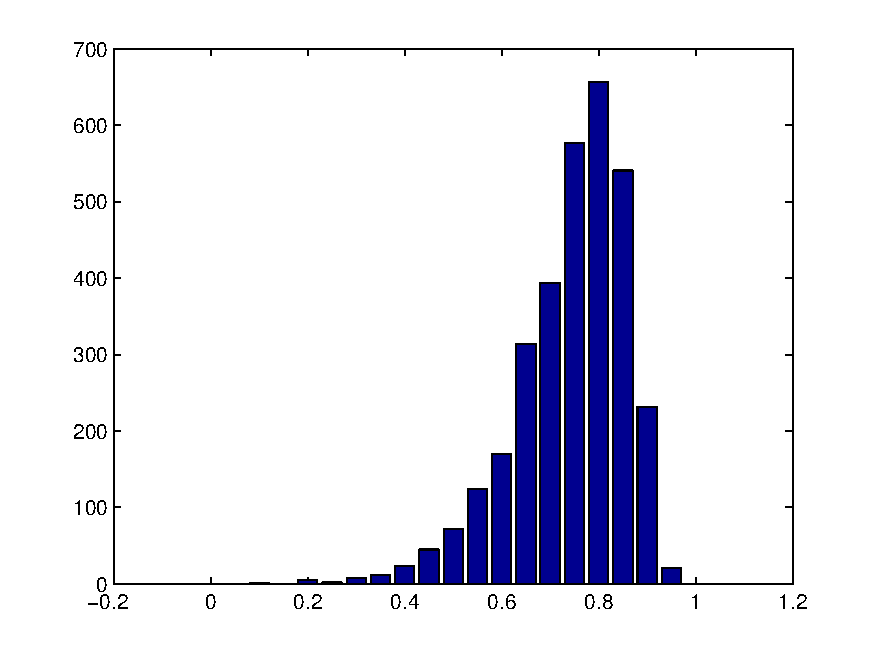
\includegraphics[width=\linewidth]{correlationparametricbootstrap3200}
\caption{Histogram of 3200 parametric bootstrap replication of corr $\widehat{\mathrm{corr}}(x^{*},y^{*})$.}
\end{figure}

\end{columns}
}

%%%%%%%%%%%%%%%%%%%%%%%%%%%%%%%%%%%%%%%%%%%%%%%%%%%%%%%
\frame{
\frametitle{The Law school example: Conclusion}

\begin{itemize}
\item The textbook formula for  the correlation coefficient is:
$$
\mathrm{se}_{\hat{f}}=(1-\widehat{\mathrm{corr}}^2)/\sqrt{n-3}
$$
With $\widehat{\mathrm{corr}}(\mathbf{x},\mathbf{y})=0.7764$, the standard error is $se_f=0.1147$.
\item The non-parametric bootstrap  standard error for $B=3200$ is $0.132$.
\item The parametric bootstrap  standard error for $B=3200$ is $0.1169$.

\end{itemize}

}


%%%%%%%%%%%%%%%%%%%%%%%%%%%%%%%%%%%%%%%%%%%%%%%%%%%%%%%%
\frame{
\frametitle{Parametric and nonparametric bootstrap estimates}

\begin{itemize}
\item The nonparametric approach leads to a finite number of possible replications $\hat{\theta}^{*}(b)$. In fact considering $n$ distinct values in $\mathbf{x}=(x_1,\cdots,x_n)$, the maximum number of \textit{different} bootstrap samples (and replications) is \footnote{$n=11$, $B_{max}=652716$: big enough to minimize the effect of the discreteness in the nonparametric approach.}:
$$
B_{max}=\left(
\begin{array}{c}
2n-1\\
n-1\\
\end{array}\right)=\frac{(2n-1)!}{n! (n-1)!}
$$     
\item The parametric approach has an unlimited number of different bootstrap samples and replications.
\end{itemize}

}
%%%%%%%%%%%%%%%%%%%%%%%%%%%%%%%%%%%%%%%%%%%%%%%%%%%%%%%%%%%%%%%%%%%%%%%%%%
\frame{
\frametitle{When might the (parametric and non parametric) bootstrap fail?}
Bootstrap might fail when:
\begin{itemize}
\item incomplete data (missing data) : incomplete observation $\mathbf{x}$
\item dependent data (e.g. correlated time series) $\mathbf{x}=(x_1,\cdots,x_n)$ dependent
\item dirty data (outliers) : noisy observation $\mathbf{x}$
\end{itemize}

\begin{block}{}
For a critical view on bootstrap, see the publication \textit{Exploring the limits
of bootstrap} edited by Le Page and Billard 1990 (ISBN: 0-471-53631-8).
\end{block}
}

%%%%%%%%%%%%%%%%%%%%%%%%%%%%%%%%%%%%%%%%%%%%%%%%%%%%%%%%
\frame{
\frametitle{Conclusion}
\begin{itemize}
\item In  parametric bootstrap, $\hat{f}_{par}$ is not anymore the empirical density function.  

\

\item If the prior information on $f$ is accurate, then  $\hat{f}_{par}$ estimates better $f$ than the empirical p.d.f.. In this case the parametric bootstrap gives better estimation for the standard errors.

\

\item Most of the time, the point  of making assumptions is to derive the textbook formulas.  \\

\textit{All models are wrong, but some are useful}- G.E.P. Box, 1979.

\

\item On the other hand, non-parametric bootstrap allows the computation of accurate standard errors (in many cases) without making any prior assumption.
\end{itemize}
}
%%%%%%%%%%%%%%%%%%%%%%%%%%%%%%%%%%%%%%%%%%%%%%%%%%%%%%%%
\frame{
\frametitle{Conclusion}
\begin{itemize}
\item In non-parametric mode, the bootstrap method relieves the analyst from choosing a parametric assumption about the form of the underlying density function $f$.

\

\item In both case, bootstrap can provide answers for problem for which no textbook formulae exists.
\end{itemize}
}
